The results of sweeping over all values of $p$ and $q$ are given in the surface plot as shown in Figure \ref{fig:allpq3d}. As expected, there are peaks when both the values are either $0$ or $1$. This is because of the the capacity is maximum where there is either no error or the channel acts as a logical NOT. This is also an ideal case, as a simple negation would provide no error. When the probabilities are $0.5$, the channel behaves randomly and hence cannot be used as a good transmission medium. Hence there is a dip in the values along the diagonal. When the transition probabilities are $0$ and $1$ or vice-versa, all the bits received are the same. This also makes the channel impractical for transmission.

The sudden peaks seem to be due to MATLAB calculation practicalities. Figure \ref{fig:allpq2d} makes it easier to look at the capacity values over $p$ and $q$ and also highlights the specific value of $q$ that is required for analysis.

\begin{figure}[h!]
    \centering
    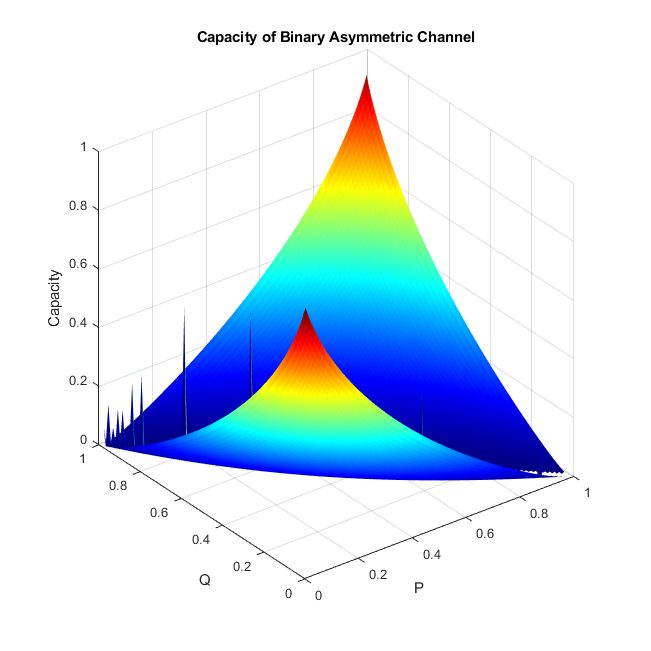
\includegraphics[width=0.4\textwidth]{images/allq1.png}
    \caption{Sweeping Across P and Q}
    \label{fig:allpq3d}
\end{figure}

\begin{figure}[h!]
    \centering
    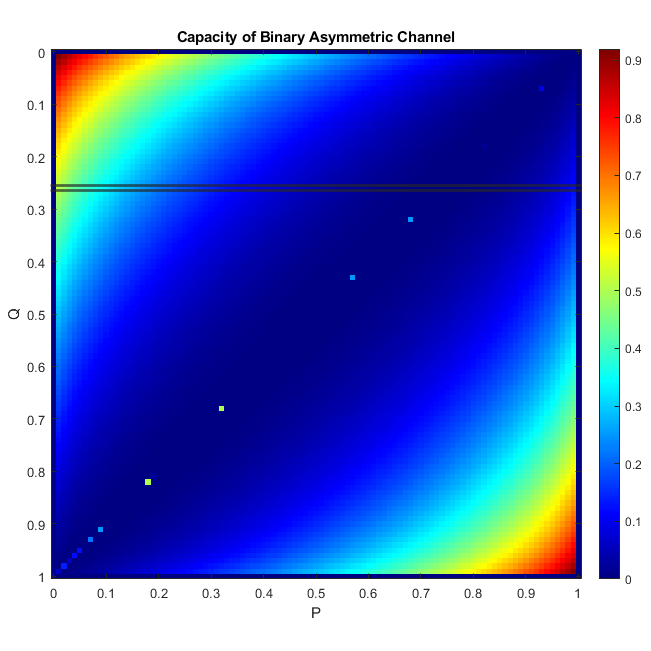
\includegraphics[width=0.4\textwidth]{images/allq2.png}
    \caption{Sweeping Across P and Q}
    \label{fig:allpq2d}
\end{figure}

As seen, the channel capacity varies along p and has peaks at either transition probabilities as $0$ and $1$ which is the expected behavior as the transition probabilities are independent of each other. Once the transition probability of one of the input symbols is fixed. The capacity is maximized when the transition probability of the second symbol is either $0$ or $1$.

Figure \ref{fig:comparison} shows the comparison of the Capacity of a Binary Asymmetric Channel with independent transition probabilities with that of Binary Symmetric Channel and Z Channel. The dotted lines show the Capacity of the compared channels when the transition probabilities are fixed to $0.26$ as required and the continuous lines show the Capacities when the probabilities are varying.

\begin{figure}
    \centering
    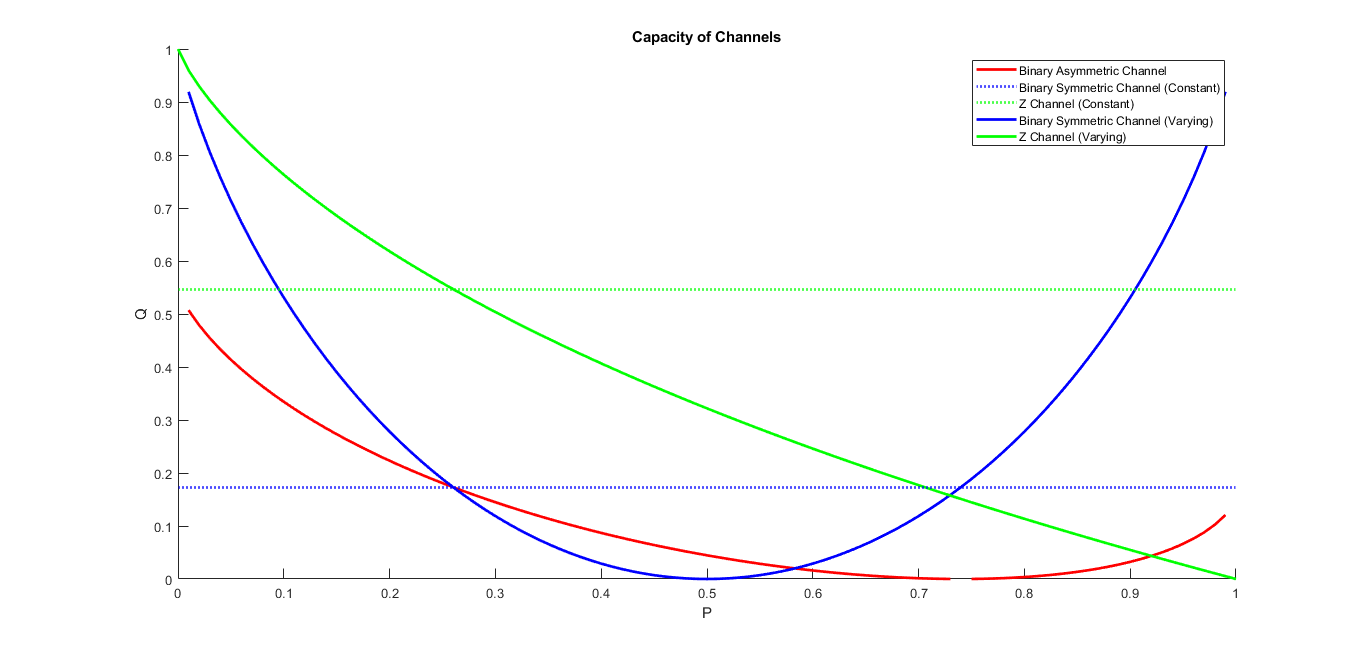
\includegraphics[width=0.5\textwidth]{images/comparison.png}
    \caption{Comparing with Channels}
    \label{fig:comparison}
\end{figure}

Consider the varying BSC, in general the Capacity of the channel is better compared to the channel under observation but when the transition probability is $0.5$, the BSC has $0$ Capacity while the BAC has a non-zero capacity. This is due to the skew in the probabilities of the the second transition which lets the user transmit with some level of confidence. The BSC with fixed probability performs well when compared to the BAC at higher transition probabilities because the value of $q$ is very low, which makes the appearance of 1 at the output much more likely. This decreases the overall capacity.

The varying Z Channel performs well at lower levels as lower transition probabilities makes the channel closer to an ideal one. But as the transition probability gets close to $1$, The BAC performs better and the Z Channel only transmits $0$. The Z Channel with constant transition probability performs much better as $0.26$ is comparatively a small transition probability and drops the capacity to around three-fourth the maximum value.